\chapter{Language Analysis}
\label{chap:language_analysis}
To get a better idea of the landscape of educational programming languages, we are going to compare three popular educational languages.
The three languages are: Scratch, BlueJ and Dr. Racket.
These three languages are chosen as the most popular learning environments for languages of each their paradigms \todo{probably need to find a source for such a claim}.
Scratch represents an imperative paradigm, BlueJ an object-oriented paradigm and Dr. Racket a functional paradigm.

In this chapter a subjective comparative analysis is made of the three programming environments/languages; Scratch, BlueJ and Dr. Racket. The procedure used for the analysis is as follows: First, some tasks have been made which are implemented in the different environments/languages. Then each language is analyzed individually using the implementations of the tasks, where the analysis is based on the criteria presented in \chapref{chap:criteria}. Finally, the analyses are used to compare the environments/languages in \chapref{chap:results}. \todo{Depends on where we make the final comparison.} The goal of this analysis is to get an insight into what each paradigm has to offer regarding educational programming and their environment and how they compare. \todo{We all need to agree that this is the case.}

The tasks are made to get as good an overview of the languages as possible. They will sometimes hypothetically favor a certain paradigm over the other, but this is done on purpose to try and find possible problems with the languages. The tasks that are implemented in each of the languages are:
\begin{description}[style=nextline]
\item[Task 1: Iterator] This task is to create a list of a certain size, which is filled with random numbers between 0 and 19, and to create a function which adds a number to every other element in the list. The purpose of this task is to get an example of how lists are made and iterated through in the different languages, which also will give an idea of how the languages are structured in general.
\item[Task 2: Fibonacci Sequence] This task is to implement an algorithm which calculates numbers of the Fibonacci sequence limited by an input by a user. The purpose of this task is to see how an ``introductory'' algorithm can be implemented in each language. It is also to have a task that somewhat favors the functional paradigm, as the functional paradigm is meant to be away to express math in a programmatic way.
\item[Task 3: Cups and Ball] This task is to create a game where a ball is hidden under a cup with 15 cups to choose from, and the goal is to locate the ball. The purpose of this task is two fold, where the first part is to show how the interactive window work in Scratch and the second part is to have a task that hypothetically favors object oriented languages, and to see how this is coped with in a non-object oriented language. Two of the three environments/languages does not support graphics as such, so there will be a difference in how this task is handled in between the languages.
\item[Task 4: Hangman] This task is to create a hangman game, where the user is supposed to guess a word with only a set amount of wrong guesses. The purpose of this task is to have a larger piece of software as the precious tasks are quite small in a sense. This will hypothetically favor Scratch and BlueJ over Dr. Racket, as the functional paradigm is not really meant for this sort of task.
\end{description}
\section{Scratch}
\label{sec:scratch}

Scratch Is chosen as the imperative language, and as the visual representative of the programming languages. As this causes the language to differ in both paradigm and writing style, it also affects the discussion on the criteria. Hence, there will be a focus on both aspects that differs from the other chosen languages.

\subsection{Iterator}
The iterator is made in a standard iterative way, through a simple loop. The debugging tool when clicking a piece of code is used to show a visual representation of the output in the game window. The control structure is a \emph{repeat} loop, which is the same as the well known \emph{for} loop, only with another name. The code for the program can be seen in \figref{fig:scratch_iter_code}, and the output is seen in \figref{fig:scratch_iter_out}.

\begin{figure}[h]
  \centering
    \begin{subfigure}[b]{0.45\textwidth}
    \begin{center}
      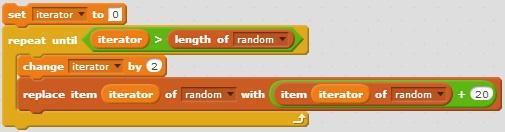
\includegraphics[scale=0.5]{./pics/scratch_iter_code}
      \caption{Scratch Iterator code.}
      \label{fig:scratch_iter_code}
    \end{center}
    \end{subfigure}
    ~
    \begin{subfigure}[b]{0.45\textwidth}
    \begin{center}
      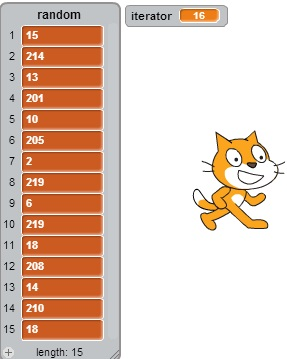
\includegraphics[scale=0.5]{./pics/scratch_iter_out}
      \caption{Scratch Iterator output.}
      \label{fig:scratch_iter_out}
    \end{center}
    \end{subfigure}
    \caption{Code and output for Hangman.}
    \label{fig:scratch_iter}
\end{figure}

\subsection{Fibonacci}
The fibonacci sequence is done through simple iteration in Scratch. An example can be seen in \figref{fig:scratch_fibo_code}. The user is asked to input how many numbers of the sequence are wanted. With a single loop and a selection, a list is presented, as seen in \figref{fig:scratch_fibo_out}.

\begin{figure}[h]
  \centering
    \begin{subfigure}[b]{0.45\textwidth}
    \begin{center}
      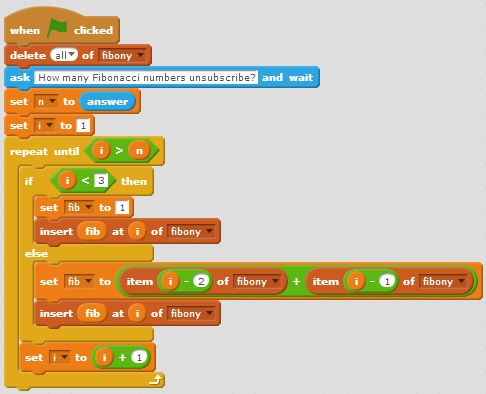
\includegraphics[scale=0.7]{./pics/scratch_fibo_code}
      \caption{Scratch fibonacci code.}
      \label{fig:scratch_fibo_code}
    \end{center}
    \end{subfigure}
    ~
    \begin{subfigure}[b]{0.45\textwidth}
    \begin{center}
      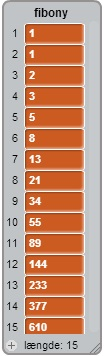
\includegraphics[scale=0.6]{./pics/scratch_fibo_out}
      \caption{Scratch fibonacci output.}
      \label{fig:scratch_fibo_out}
    \end{center}
    \end{subfigure}
    \caption{Code and output for fibonacci numbers.}
    \label{fig:scratch_fibo}
\end{figure}

\subsection{Cups and Ball}
The game of guessing the position of the ball amongst the cups is made with events, as Scratch is able to handle these with blocks. Events happen e.g. when a cup is clicked, cups are cloned, and when the ball is clicked. Code is also attached different sprites, as these work individually to the events. The code blocks for the cups can be seen in \figref{fig:scratch_ball_code1}, and the code blocks for the ball can be seen in \figref{fig:scratch_ball_code2}. A screenshot of the game screen while in a game can be seen in \figref{fig:scratch_ball_out}.

\begin{figure}[h]
  \centering
    \begin{subfigure}[b]{0.45\textwidth}
    \begin{center}
      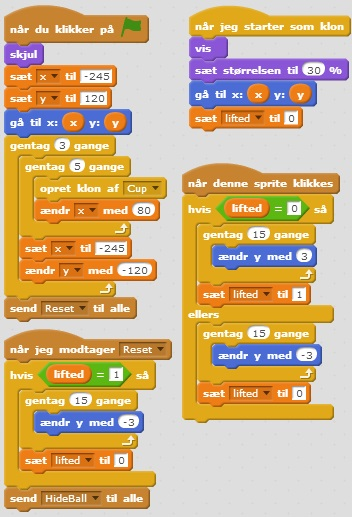
\includegraphics[scale=0.7]{./pics/scratch_ball_code1}
      \caption{Scratch cup code.}
      \label{fig:scratch_ball_code1}
    \end{center}
    \end{subfigure}
    ~
    \begin{subfigure}[b]{0.45\textwidth}
    \begin{center}
      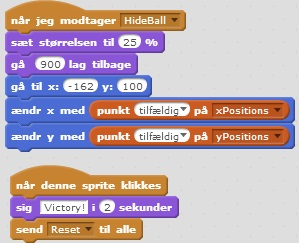
\includegraphics[scale=0.7]{./pics/scratch_ball_code2}
      \caption{Scratch ball code.}
      \label{fig:scratch_ball_code2}
    \end{center}
    \end{subfigure}
    
    \begin{subfigure}[b]{\textwidth}
    \begin{center}
      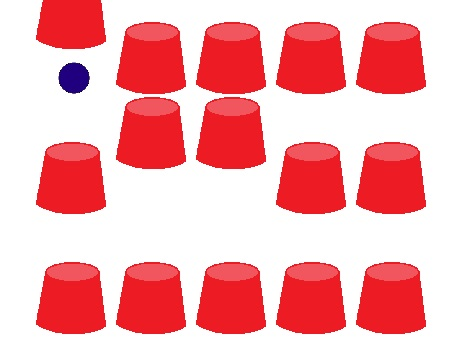
\includegraphics[scale=0.5]{./pics/scratch_ball_out}
      \caption{Scratch Cups and Ball output.}
      \label{fig:scratch_ball_out}
    \end{center}
    \end{subfigure}
    \caption{Code and output for Cups and Ball.}
    \label{fig:scratch_ball}
\end{figure}

\subsection{Hangman}
The Hangman game is made in an imperative manner. As there are many conditions to take into account, the code is rather long, and there is a lot of control structures. The guessing part itself is a big loop, which can be seen in \figref{fig:scratch_hang_code}. On the game screen, a list holds the letters for the word to guess, a list holds all the wrong guesses, and a sprite changes for each wrong guess. An input field is provided for guessing. The game screen can be seen in \figref{fig:scratch_hang_out}.

\begin{figure}[h]
  \centering
    \begin{subfigure}[b]{0.45\textwidth}
    \begin{center}
      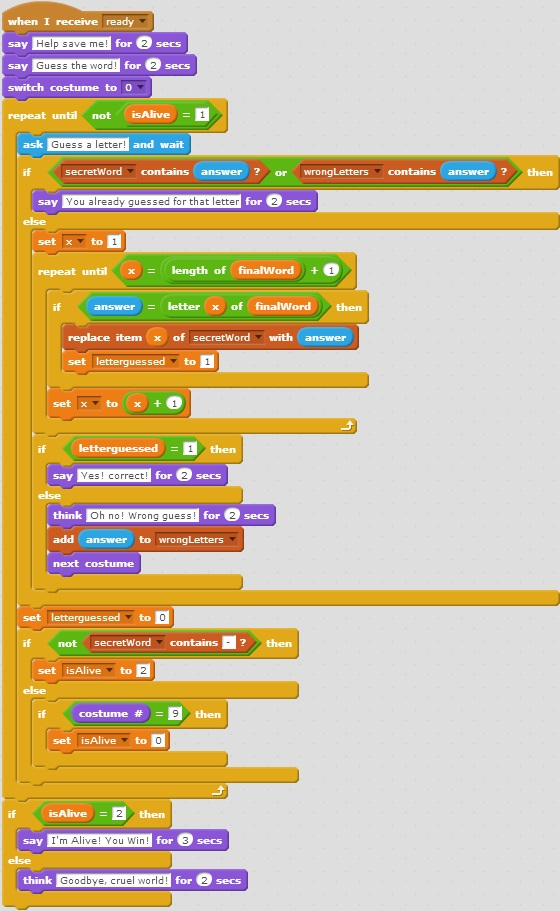
\includegraphics[scale=0.5]{./pics/scratch_hang_code}
      \caption{Scratch Hangman code.}
      \label{fig:scratch_hang_code}
    \end{center}
    \end{subfigure}
    ~
    \begin{subfigure}[b]{0.45\textwidth}
    \begin{center}
      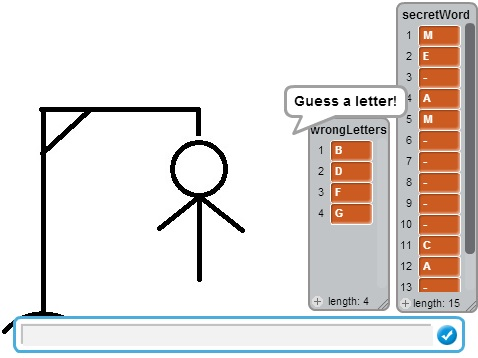
\includegraphics[scale=0.5]{./pics/scratch_hang_out}
      \caption{Scratch Hangman output.}
      \label{fig:scratch_hang_out}
    \end{center}
    \end{subfigure}
    \caption{Code and output for Hangman.}
    \label{fig:scratch_hang}
\end{figure}

\subsection{Criteria Evaluation}

\begin{description}[style=nextline]
\item[Readability] Scratch is known for its great readability, and this shows when reading it. The colored structures clearly show what the different building blocks are doing. This could lead to a problem with color blind people, as it is not possible to change the colors. The language is very verbose in its statements and declarations, leading to a better understanding of what happens in a block. A problem is the fact that a project becomes very big very fast. An example of this can be seen in \figref{fig:scratch_hang_code}, where the collection of blocks seems hard to read at first glimpse, due to its sheer size.
\item[Writability] The visual programming style has its pros and cons. It is easy to create simple structures, but it takes too long for an advanced programmer. It is extremely easy to understand how to use Scratch, due to the fact that it uses building blocks as arguments.
\item[Observability] Scratch has a live game window, where output is shown when compiling code. Combined with the possibility of double-clicking sets of blocks to compile that specific piece of code, the programmer can see the output whenever wanted.
\item[Trialability] The visual environment in Scratch allows close to no syntax errors. Combined with the level of observability, Scratch has great possibility of recovering from errors, as the error is easily found in the game window. In bigger programs, however, it can be hard to find the error, as one cannot follow the stack. Closing in on a small error that affects the whole program can be hard.
\item[Learnability] Making a game is a good way to capture the attention of children. But to keep them occupied, the process of coding should be intensive in a playful way. Building blocks from the visual style is a way to do it, as building blocks has been proven successful in the context of playing (Lego is an example of this). The lack of conventional syntax, however, can be hindering further in the programmer's career. That means the language is great for novice programming, but it comes to a stop.
\item[Reusability] As Scratch is also a minor game engine, it uses 2D sprites for visualization. Each sprite can contain code local to that sprite. The code shown in \figref{fig:scratch_ball_code1} is the code local to the Cup sprite, whereas the code shown in \figref{fig:scratch_ball_code2} is local to the Ball sprite. As these can be cloned, the code written serves as a blueprint for all instances of the sprite to use. Furthermore, Scratch has the possibility of defining custom blocks. These blocks can bring a collection of blocks down to the size of one, and they can easily be reused. These custom blocks work as functional procedures for the language.
\item[Pedagogic Value] Scratch makes use of the most basic of concepts, such as variables and control structures. That said, there is a huge leap when moving from Scratch to a non-visual programming language. The lack of conventional syntax, which is found in text based programming languages, can confuse a novice when moving on.
\item[Environment] Scratch has a very friendly environment, with great visibility in the color coding. As novices are not familiar with anything code-related, the naming of structures is meaningful and easy to understand. Navigation can be a bit confusing at first, as it can be hard to know what category a needed block is found in. The control of the blocks can be a bit annoying, as disconnecting interlocked blocks does not always go as expected. The game window combined with the block compilation, as mentioned, is a great way of obtaining feedback for trial-and-error.
\item[Documentation] Scratch has an integrated introduction tutorial, which is a great way for novices to learn the language. Furthermore, each building block can be right-clicked to find a documentation page for that specific block. This documentation is easy to read, but is unfortunately only available in English. Furthermore, it is possible to find and share projects via Scratch's homepage.
\item[Uniformity] The basic concepts used in Scratch do the same as in other languages. However, the naming of the expressions and structures are often different, e.g. Scratch has a \emph{repeat} structure, instead of a \emph{for} structure.
\item[Miscellaneous] Scratch uses sprites, but it is very hard to make different sprites work together, as the language itself is not object-oriented. As an example, you cannot reference to a specific sprite or one of its clones. Furthermore, the language has great accessibility in the fact that it is programmed in a browser.
\end{description}
\section{BlueJ}
\label{sec:bluej}

\todo{Results and discussion.}


Since BlueJ uses Java as its underlying language, all the selected tasks will be implemented in imperative, object-oriented manner and there also might be some similarities to their counterparts in Scratch in terms of code structure and use of constructs.
\subsection{Iterator}
The Iterator in BlueJ is implemented using simple iteration through a list with a certain size, specified by the user. Then a \textit{for} loop is used to add a number,in that case 20, to every other element from that list and then the result is printed, as shown in \figref{fig:bluej_iterator_code}

\begin{figure}[!h]
  \centering
      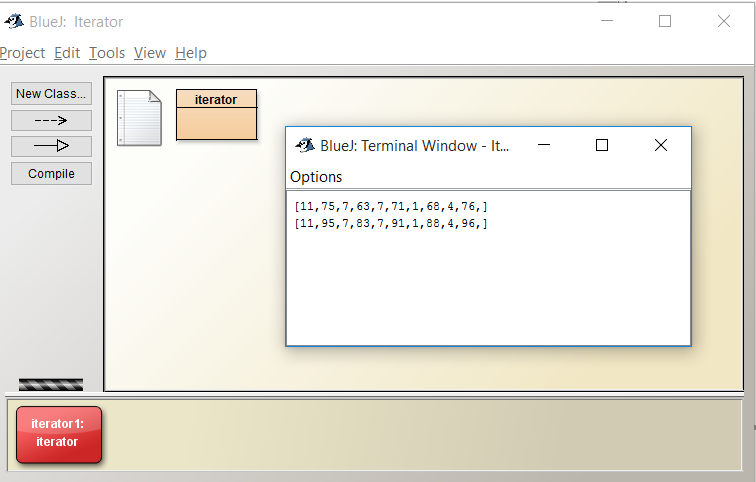
\includegraphics[scale=0.7]{./pics/bluej_iterator_code}
      \caption{Code and output for Iterator}
      \label{fig:bluej_iterator_code} 
\end{figure}

\subsection{Fibonacci}
The Fibonacci sequence in BlueJ can be expressed both by using an iterative and recursive approaches. An example could be seen in \figref{fig:bluej_fibo_code2}, where the user is prompted to give a number and the respective result is shown.

\begin{figure}[!h]
  \centering
    \begin{subfigure}[b]{0.45\textwidth}
    \begin{center}
      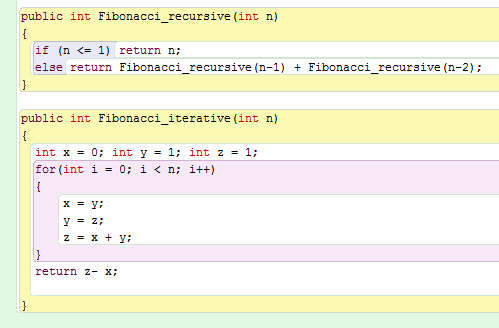
\includegraphics[scale=0.7]{./pics/bluej_fibo_code}
      \caption{BlueJ Fibonacci code.}
      \label{fig:bluej_fibo_code}
    \end{center}
    \end{subfigure}
    ~
    \begin{subfigure}[b]{0.45\textwidth}
    \begin{center}
      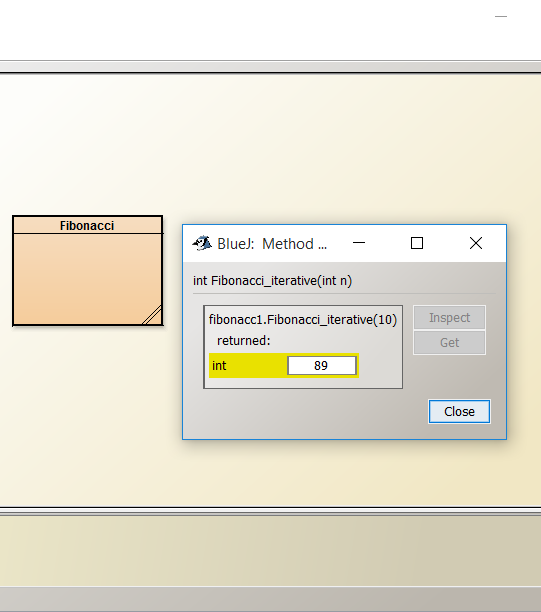
\includegraphics[scale=0.6]{./pics/bluej_fibo_code2}
      \caption{BlueJ Fibonacci output.}
      \label{fig:bluej_fibo_code2}
    \end{center}
    \end{subfigure}
    \caption{Code and output for Fibonacci numbers.}
    \label{fig:bluej_fibo}
\end{figure}
\subsection{Cups and Ball}
Similarly to how this game was implemented in Scratch, it gives the player the chance to guess where a ball might be among 15 identical cups, with the difference that it feels less intuitive since there is no visual feedback given but rather textual one - that the player has either successfully guessed the position of the ball or not. The example can be seen in \figref{fig:bluej_ballcup_code} 

\begin{figure}[!h]
  \centering
      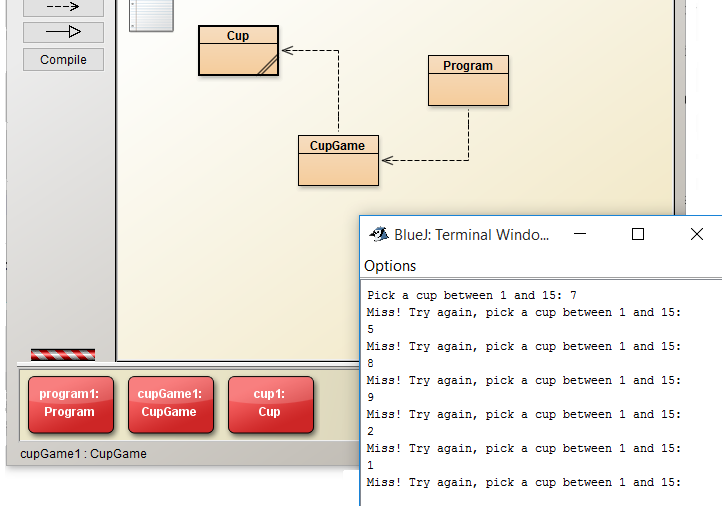
\includegraphics[scale=0.7]{./pics/bluej_ballcup_code}
      \caption{Code and output for Cups and Ball}
      \label{fig:bluej_ballcup_code} 
\end{figure}

\subsection{Hangman}
The Hangman is also a guessing game where the player has to guess a particular word by providing one letter at the time. In BlueJ implementation, if the letter is part of the word, the its added to a guessing list, otherwise if it not, it is added to a wrong list instead. Every time the player gives a wrong letter, one of his lives is lost, thus the "total lives" the counter decrements by one, and if he is to lose all of them eventually, the game is lost and he has to start all over. The code follows an imperative style of programming with conditional statements and loops, some of which are illustrated on \figref{fig:bluej_hangman_code} 

\begin{figure}[!h]
  \centering
      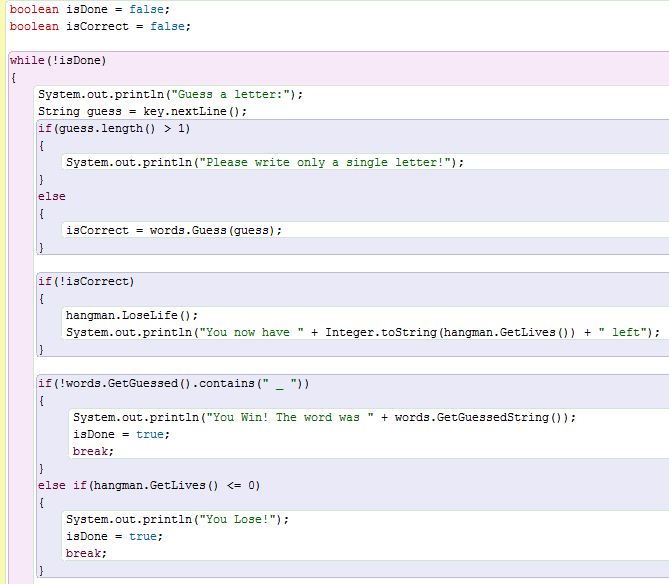
\includegraphics[scale=0.7]{./pics/bluej_hangman_code}
      \caption{Code for Hangman game}
      \label{fig:bluej_hangman_code} 
\end{figure}

\subsection{Criteria Evaluation}
\begin{description}[style=nextline]
\item[Readability]
BlueJ has sufficiently good readability both by its textual and visual representations. The Main panel provides an overview of the hierarchy and interactions between different classes and objects giving novice programmers a greater understanding of how different pieces of the code are connected. Additionally, the textual representation provides good indentation and different colour schemes for every method so it is easier to understand the structure of the code.
\item[Writability]
As already mentioned in Section \ref{sec:bluej}, BlueJ uses Java as its underlying language, therefore it inherits all its pros and cons along. Writing code follows an object-oriented fashion and additionally keywords, such as data types, return statements etc., are highlighted in order to be differentiated by the programmer more easily.
\item[Observability]
BlueJ has fairy good observability as it usually manages to quickly and efficiently compile the code giving more time to test different scenarios since it is mainly suitable for small educational projects. Its visual representation provides the option to create instances of objects as visual elements and call different methods specific to these objects in an easy, fast and understandable way.  
\item[Trialability]
In terms of trialability, BlueJ has a good handling of syntactical and semantic errors, where the need be exceptions are thrown and the code cannot be compiled before those are fixed. Additionally, the problematic sections are highlighted in red with an appropriate message for the give error.
\item[Learnability]
Since BlueJ is first and foremost an educational platform, it provides a good way for novice programmers to jump into the object-oriented style of programming with a steady learning curve and sufficiently good documentation.
\item[Reusability]
BlueJ provides a great deal of reusability as it is fairly simple to drag and drop classes from other projects and integrate them into the existing one with small modifications. 
\item[Pedagogic Value]
BlueJ is a powerful educational tool which provides a gentle introduction for novice programmers to the world of object-oriented programming. Given its thorough documentation and exercises with steadily increasing difficulty, BlueJ can give a solid start for everyone with the aptitude for learning.
\item[Environment]
Usually, the Integrated Development Environment (IDE) of a language is the only direct way of communication with that language. In the case of BlueJ, it provides the bare essentials needed for learning object orientation, specifically targeting novice programmers without the unnecessary clutter present in more advanced IDEs such as Eclipse or NetBeans. Furthermore, it does not require much effort to install it and create projects in it.
\item[Documentation]
As already mentioned, BlueJ has a solid documentation with a lot of reference materials and additional exercises for those who are interested to delve deeper in its features. Also it is fairly easy to get access to the documentation on the BlueJ homepage without the need for any additional books.
\item[Uniformity]
BlueJ has a high uniformity compared to other languages since Java is a widespread language and it uses well established language constructs. Its language constructs have mostly predictable behaviour.
\end{description}
\section{DrRacket}
\label{sec:drracket}
DrRacket is an environment used to learn to write Racket code.
Racket is a functional programming language, and therefore DrRacket is our representative for an educational programming environment for the functional paradigm.
Worth noting is that all of of the authors have learned to program in an imperative paradigm first and do not have much experience working with functional languages.
This will likely impact the code examples as well as the opinions in the criteria evaluation.

\subsection{Iterator}
The first code example is the iterator example.
In functional programming, when one wants to apply a function through a list, one would usually use the map function. However, since that applies the function to every element in the list, and we want to apply it to every other element the code looks like shown in \lstref{DrRacket_iterator} instead.

\begin{lstlisting}[caption={The iterator function in DrRacket}, label={DrRacket_iterator}]
(define (iterator inList)
  (if (< (length inList) 2)
      inList
      (cons (car inList) (cons (+ (car(cdr inList)) 20) (iterator (cdr(cdr inList)))))))
\end{lstlisting}

The function takes a list \lstinline!inLinst! in and returns a list.
In the trivial case where the list is shorter than two, the function does not need to be applied to anything and the list is simply returned.
Otherwise the second element in the list should be modified and the function recursively called on the remainder.
To do this three functions are used:
\lstinline!car! which returns the first element of the list called the head, \lstinline!cdr! which returns the list minus the first element called the tail, and \lstinline!cons! which combines a head and a tail to create the bigger list.
Firstly we want to combine the unmodified head of the list with the modified tail to construct the new list.
We then construct the modified tail by modifying the head of the tail, which modifies the second element in the list, and calling the function recursively on the tail of the tail to go through the rest of the list, and combining these.

\subsection{Fibonacci}
The second example is shown in \lstref{DrRacket_fibonacci}. 
This is a simple recursive implementation of Fibonacci with no memory optimizations.
Recursion is second nature to functional programming languages, so this is an intuitive implementation.
The function takes in a number to find the Fibonacci number of and then calls itself recursively on the two preceding numbers to get the two numbers it needs to sum up.
Eventually a trivial case of the called number being one or zero in which case it simply returns one.

\begin{lstlisting}[caption={The Fibonacci function in DrRacket}, label={DrRacket_fibonacci}]
(define (fibonacci n)
  (if (or (= n 0) (= n 1))
      1
      (+ (fibonacci (- n 1)) (fibonacci (- n 2)))))
\end{lstlisting}

\subsection{Cups and Ball}
The next code example is the cups and ball example.
This example is intuitively solved in an object-oriented way and since Racket has objects and classes, we do it like that.
The definition of the class \lstinline!Cup! can be seen in \lstref{DrRacket_cup_object}. Each object of the class has a variable \lstinline!holdsBall!, which is used to store whether this cup has a ball, used as a boolean.
They also have two functions: \lstinline!AddBall! which sets \lstinline!holdsBall! to 1, and \lstinline!HasBall! which returns \lstinline!holdsBall!.
The code then creates a list of 15 balls and calls \lstinline!AddBall! on one of them chosen randomly.
The main game loop is facilitated with a recursive function \lstinline!AskUser!, which is shown in \lstref{DrRacket_AskUser}.
Here the user is prompted for a number between 1 and 15.
The cup on that position on the list then has its \lstinline!HasBall! function called.
If it is 1 the user is congratulated and the game ends, otherwise the user is prompted to guess again and the \lstinline!AskUser! function is called to repeat the cycle.

\begin{lstlisting}[caption={The Cup class definition in DrRacket}, label={DrRacket_cup_object}]
(define Cup%
  (class object%
    (define holdsBall 0)

    (super-new)
    
    (define/public (AddBall)
      (set! holdsBall 1)
      )
    
    (define/public (HasBall)
      holdsBall)
))
\end{lstlisting}

\begin{lstlisting}[caption={The AskUser function in DrRacket}, label={DrRacket_AskUser}]
(define (AskUser)
   (define guess (read))
  (if (= (send (list-ref cups (- guess 1)) HasBall) 1)
      (println "Congratulation, you found it!")
     (begin
       (println "Miss! Try again, pick a cup between 1 and 15: ") (AskUser))))
\end{lstlisting}



\subsection{Hangman}
The final example is the game of hangman.
Here we have a list of 11 words all 15 letters long represented by strings. The initial values are then defined:
\begin{itemize}
\item \lstinline!finalWord! is assigned a random string from our list of words and represent the word that should be guessed
\item \lstinline!wrongLetters! represent the list of letters guessed on that were wrong and is assigned to the empty list
\item \lstinline!knownLetters! is the list of correctly guessed letters and their position. This is initialized to a mutable string of 15 underscores.
\item \lstinline!hangman! is the number of lives left and it is initialized to 8.
\end{itemize}

The user can guess on a letter by calling the guess function with a string.
If the string is one char long the function \lstinline!checkLetter! is called with parameters 0 and the guess string. The function can be seen in \lstref{DrRacket_checkLetter}.

\begin{lstlisting}[caption={The checkLetter function in DrRacket}, label={DrRacket_checkLetter}]
(define (checkLetter st l)
  (cond
    [(> (+ st 1) (string-length finalWord))
     (if (and (equal? hasFound 0) (not (member l wrongLetters)))
         (loseLife l)
         #f)]
    [(equal? l (substring finalWord st (+ st 1)))
     (printf "correct guess! on place ~a\n" (+ st 1))
     (set! hasFound 1)
     (string-set! knownLetters st (string-ref l 0))
     (checkLetter (+ st 1) l)
     #t]
    [else (checkLetter (+ st 1) l)]))
\end{lstlisting}

The \lstinline!st! parameter is the index of the char in the \lstinline!finalWord! string we are looking at and \lstinline!l! is the guess string.
This function checks for three conditions:

\begin{itemize}
\item If the index is larger than the length of the string, we are done going through the string.
\lstinline!hasFound! is initialized in \lstinline!guess! to 0 and if it hasn't changed it means the letter was not found in \lstinline!finalWord!.
If \lstinline!l! also was not in the \lstinline!wrongLetters! list, it means the guess was a new wrong guess and \lstinline!loseLife! is called.
\lstinline!loseLife! reduces \lstinline!hangman! by one and adds the letter to \lstinline!wrongList!.
\item If \lstinline!l! is equal to the substring of \lstinline!finalWord! at index \lstinline!st! then the guess is correct.
The user is notified, \lstinline!hasFound! is set to 1, the letter at index \lstinline!st! in \lstinline!knownLetters! is changed to \lstinline!l! and the function is called recursively on the next index to go through the rest of the string.
\item Otherwise the function is called with the next index to keep looking through the string.
\end{itemize}

In the end the function \lstinline!guess! checks for \lstinline!hangman! being 0 to report a loss and if underscore is still a part of \lstinline!knownLetters! as otherwise a win is reported.

\subsection{Criteria Evaluation}
\label{subsec:criteval}
In this section we will discuss DrRacket in relation to our criteria. Again, since the authors are used to another programming paradigm, these opinions might be biased.

\begin{description}[style=nextline]
\item[Readability] DrRacket is fairly readable, with the mandatory use of parentheses giving it a certain structure.
The heavy use of parentheses however does mean that they sometimes can blend together making it harder to distinguish the operations from each other as can be seen in \lstref{DrRacket_iterator}.
The environment does provide an automatic highlight of the area a pair of parentheses cover when the cursor is next to one, but it does not fix the immediate readability.
The lack of infix operators hurts the readability since it means that common mathematical operators like plus, minus and greater-than need to be before the two arguments.
This breaks the common mathematical notation, which makes it harder to understand intuitively.
In general the functional paradigm also has some readability issues since the code usually requires a better overview of the function to understand it.
In a more imperative paradigm it is easier to build up an understanding from partial understandings of the sequences.
\item[Writability] DrRacket has good writability, often being able to express things a little more concisely and having a consistent syntax for all sorts of function calls.
There is good support for many levels of abstraction with functions being an integral part of the language and it offering constructs for object-oriented programming.
Its only problems are a the higher need for overview like in readability, and that the syntax especially around missing parentheses can get hard to keep track of and often requires some debugging.
The parentheses highlight tool does help with that quite well though.
\item[Observability] DrRacket has good observability, as it offers an immediate console on runtime, where one can call all the functions and variables from your code and immediately see the return value.
\item[Trialability] DrRacket has good trialability, as the code compiles quickly and easily and whenever an error is encountered it highlights the code it found the error as well as giving the error message.
It does have the usual issues with the error message not always being helpful and sometimes reported at other places than where the actual problem is, and you still need to compile every time you want to test any changes to the code.
\item[Learnability] DrRacket has good learnability with the possibility of using sublanguages to restrict the possibilities available to novice programmers.
This allows for slowly opening up the higher level sublanguages to build towards the full language.
It also has easily available tutorials to learn the language in this manner.
It does however have the problem of not showing the legal constructs to a novice, which means they have to look up the documentation to find examples of how the code should look.
\item[Reusability] DrRacket has great reusability with a strong focus on using functions on many levels and support for objects and classes.
\item[Pedagogic Value] DrRacket has some great pedagogical values in the way that it encourages learning and using recursion, which is a powerful programming tool.
Its consistency with function call conventions also help convey the ubiquitous use of function calls.
Notably the choice of sticking to the function call syntax instead of allowing infix operators in mathematical expressions, help convey the fact that these are coded as functions in the code.
\item[Environment] DrRacket is a reasonably good environment for Racket.
It provides easy setup of compilation to an easily accessible console to evaluate the code with.
Its tools for highlighting the parantheses areas and and marking the definition with a line to it when hovering over a variable, both help keep track of the structure.
The environment itself however does not provide any assistance for getting started.
\item[Documentation] DrRacket has a lot of good documentation both in the form of easily accessible online tutorials and an online manual with a search function.
There are also several books on the subject as well as a decent amount of online forum discussions on Racket and Scheme.
\item[Uniformity] DrRacket has low uniformity relative to the other languages we know like Java, C\# and F\#.
Its function calls has the parentheses around the whole call instead of only the parameters, and the lack of infix operators makes basic mathematical operations look vastly different.
\end{description}